% 2004 年全国卷Ⅱ文科第 20 题：直三棱柱
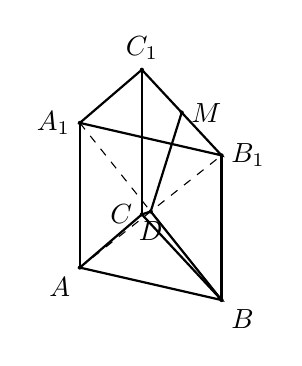
\begin{tikzpicture}[>=stealth,scale=0.75]
  \coordinate (A) at (0,0); \coordinate (B) at (2.4,-0.55);
  \coordinate (C) at (1.05,0.9); \coordinate (A1) at (0,2.45);
  \coordinate (B1) at (2.4,1.9); \coordinate (C1) at (1.05,3.35);
  \coordinate (D) at (1.2,0.95); \coordinate (M) at (1.725,2.625);
  \draw[thick] (A)--(B)--(C)--cycle;
  \draw[thick] (A1)--(B1)--(C1)--cycle;
  \draw[thick] (A)--(A1) (B)--(B1) (C)--(C1);
  \draw[dashed] (A)--(B1) (A1)--(B) (C)--(D);
  \draw[thick] (D)--(C) (D)--(B) (D)--(M);
  \fill (A) circle (1pt) node[below left] {$A$};
  \fill (B) circle (1pt) node[below right] {$B$};
  \fill (C) circle (1pt) node[left] {$C$};
  \fill (A1) circle (1pt) node[left] {$A_1$};
  \fill (B1) circle (1pt) node[right] {$B_1$};
  \fill (C1) circle (1pt) node[above] {$C_1$};
  \fill (D) circle (1pt) node[below] {$D$};
  \fill (M) circle (1pt) node[right] {$M$};
\end{tikzpicture}
